\documentclass[pdf]{beamer}

\usepackage[utf8]{inputenc}
\usepackage[T1]{fontenc}
\usepackage{graphicx}
\usepackage{tabto}
\usepackage{listings} % Required for insertion of code
\usepackage{tcolorbox}
\usepackage{subcaption}
\usepackage[main=greek, english]{babel} % For Greek language
\usepackage{tikz}
\usepackage{dirtytalk}
\usepackage{smartdiagram}
\usepackage{hyperref}
\usepackage{adjustbox}
\usetikzlibrary{shapes.geometric, arrows}
\usetikzlibrary{timeline}

\tikzstyle{startstop} = [rectangle, rounded corners, minimum width=3cm, minimum height=1cm,text centered, draw=black, fill=red!30]
\tikzstyle{io} = [trapezium, trapezium left angle=70, trapezium right angle=110, minimum width=3cm, minimum height=1cm, text centered, draw=black, fill=blue!30]
\tikzstyle{process} = [rectangle, minimum width=3cm, minimum height=1cm, text centered, draw=black, fill=orange!30]
\tikzstyle{decision} = [diamond, minimum width=3cm, minimum height=1cm, text centered, draw=black, fill=green!30]
\tikzstyle{arrow} = [thick,->,>=stealth]


\newcommand{\en}[1]{\foreignlanguage{english}{#1}}
\newcommand{\src}[1]{{\tt\en{#1}}}

\newcommand{\img}[1]
{
    \begin{center}
        \fcolorbox{black}{white}{\includegraphics[height=10em]{#1}}
    \end{center}

}

\beamertemplatenavigationsymbolsempty

\usetheme{Madrid}

\makeatletter
\setbeamertemplate{footline}{%
  \leavevmode%
  \hbox{%
    \begin{beamercolorbox}[wd=.2\paperwidth,ht=2.25ex,dp=1ex,center]{author in head/foot}%
      \usebeamerfont{author in head/foot}\expandafter\ifblank\expandafter{\beamer@shortinstitute}{}{~~(\insertshortinstitute)}
    \end{beamercolorbox}%
    \begin{beamercolorbox}[wd=.60\paperwidth,ht=2.25ex,dp=1ex,center]{title in head/foot}%
      \usebeamerfont{title in head/foot}\insertshorttitle
    \end{beamercolorbox}%
  }%
  \begin{beamercolorbox}[wd=.2\paperwidth,ht=2.25ex,dp=1ex,right]{date in head/foot}%
    \usebeamerfont{date in head/foot}%
    \usebeamertemplate{page number in head/foot}%
    \hspace*{2ex} 
  \end{beamercolorbox}
  \vskip0pt%
}
\makeatother

\title{Προγραμματισμός Διαδικτύου - \en{Project}}
\date{}
\author{Ευάγγελος Λάμπρου \and Απόστολος Παπαδημητρίου}

% \usebackgroundtemplate%
% {%
%     \includegraphics[height=\paperheight]{./template_beamer.png}%
% }

\begin{document}

\begin{frame}
    \maketitle
\end{frame}

\section{Εισαγωγή}

\begin{frame}
    \frametitle{Εφαρμοφή Υποστήριξης Κοινότητας}

    \begin{block}{Περιγραφή}
        Η εφαρμογή μας αποτελεί μία απλή υλοποίηση ενός 
        \en{forum} στο οποίο χρήστες θα μπορούν να δημιουργούν
        \en{posts}, σχόλια και να βλέπουν στατιστικά ανάλογα με τις 
        δραστηριότητές τους στην ιστοσελίδα.
    \end{block}
    
   \begin{figure}[htpb]
       \centering
        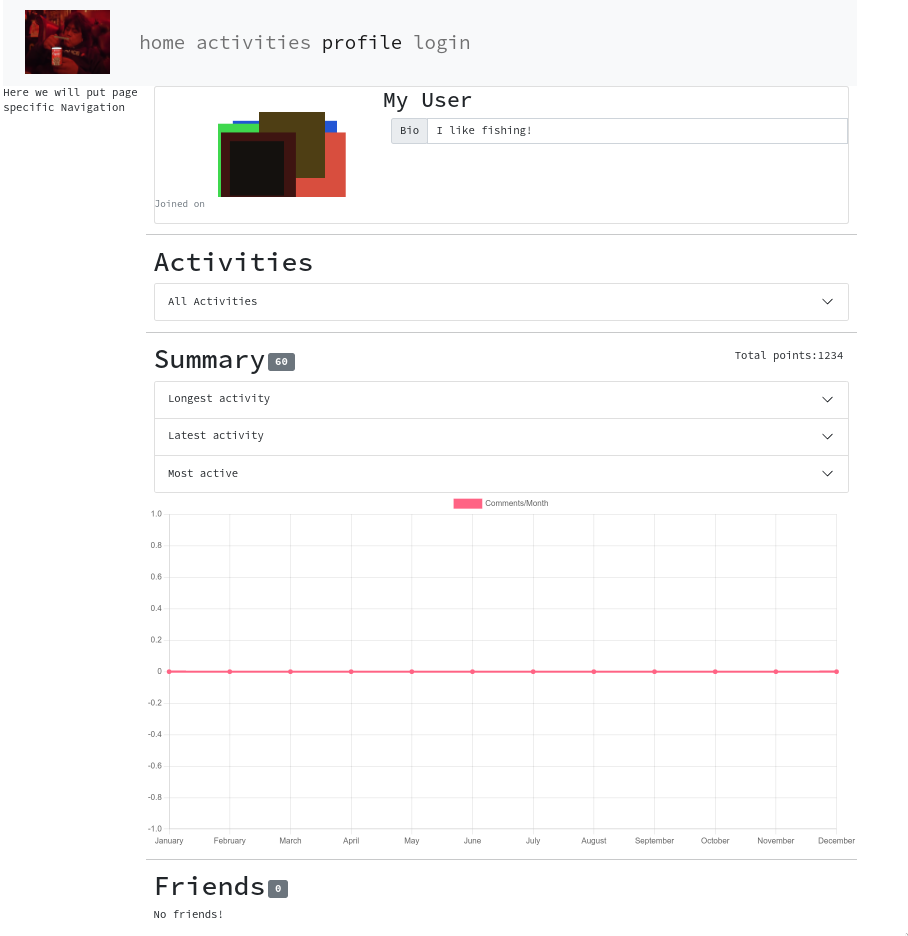
\includegraphics[width=.4\textwidth]{./assets/site.png}
   \end{figure} 
    
\end{frame}

\begin{frame}

    \frametitle{Βασικές λειτουργίες}

    \begin{itemize}
        \item Δημιουργία λογαριασμού από τον χρήστη
        \item Προσωπικό προφίλ
        \item Δημιουργία Δημοσιεύσεων / Σχόλια σε αυτές
    \end{itemize}
    
\end{frame}

\begin{frame}
    \frametitle{Ενοιολογικός Σχεδιασμός}

\begin{figure}
\begin{adjustbox}{max totalsize={.9\textwidth}{.7\textheight},center}
\begin{tikzpicture}[node distance=4.0cm, scale=0.6, every/.style={transform shape}]

    \node (start) [startstop] {Αρχική Σελίδα};

    \node (loggedin)        [decision, below of=start]         {\footnotesize Συνδεδεμένος?};
    \node (activitiespage)  [process, left of=loggedin]        {Δραστηριότητες};
    \node (postspage)       [process, below of=activitiespage] {Αναρτήσεις};
    \node (postpage)        [process, below of=postspage]      {Ανάρτηση};
    \node (profile)         [process, below of=postpage]       {Προφίλ Χρήστη};
    \node (loginpage)       [process, below of=loggedin]       {Σύνδεση};
    \node (registered)      [decision, below of=loginpage]     {\footnotesize Εγγεγραμένος?};
    \node (loginsucess)     [decision, below of=registered]    {\footnotesize Επιτυχια?};
    \node (registerpage)    [process, right of=registered]     {Εγγραφή};
    \node (personalprofile) [process, right of=loggedin]       {Προσωπικό προφίλ};

    \draw [arrow] (start)          -- (loggedin);
    \draw [arrow] (start)          -| (activitiespage);
    \draw [arrow] (loggedin)       -- node[right] {όχι} (loginpage);
    \draw [arrow] (loggedin)       -- node[above] {ναι} (personalprofile);
    \draw [arrow] (loginpage)      -- (registered);
    \draw [arrow] (registered)     -- node[above] {όχι} (registerpage);
    \draw [arrow] (registered)     -- node[right] {ναι} (loginsucess);
    \draw [arrow] (loginsucess)    -- node[right] {ναι} (personalprofile);
    \draw [arrow] (registerpage)   |- (loginpage);
    \draw [arrow] (activitiespage) -- (postspage);
    \draw [arrow] (postspage)      -- (postpage);
    \draw [arrow] (postpage)       -- (profile);
    \draw [arrow] (start)       -- (postspage);
    \draw [arrow] (start)       -- (profile);

\end{tikzpicture}
\end{adjustbox}
    \caption{Το διάγραμμα ροής χρήστη της εφαρμογής.}
    \label{fig:userflowdiagram}%
\end{figure}
\end{frame}

\begin{frame}

    \begin{figure}[htpb]
        \centering
        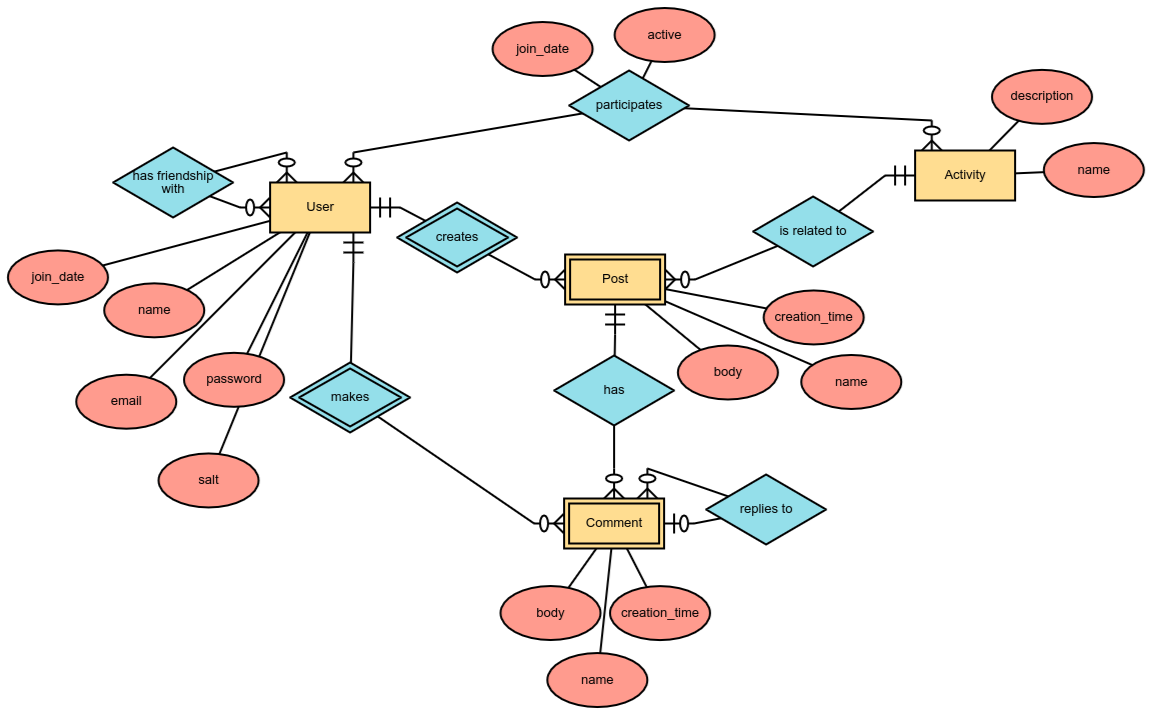
\includegraphics[width=0.8\textwidth]{./assets/erd.png}
        \caption{Το \en{ERD} της εφαρμογής.}
        \label{fig:}
    \end{figure}
    
\end{frame}


\begin{frame}
    \frametitle{\en{Tech Stack}}


\begin{figure}[htpb]

    \begin{adjustbox}{max totalsize={.9\textwidth}{.7\textheight},center}
    \smartdiagram[descriptive diagram]{
        {\en{Bootstrap}, {Έτοιμα \src{CSS/Javascript} \en{components}}},
        {\en{Handlebars}, {\src{HTML} \en{Render Engine}}},
        {\en{Express}, {\en{WebServer}}},
        {\en{Node}, {Περιβάλλον εκτέλεσης \src{Javascript}}},
        {\en{MySQL}, {\en{DataBase Management System}}},
    }
    \end{adjustbox}
    \caption{Τα βάσικα μερή του \en{technology stack} που χρησιμοποιήσαμε.}
\end{figure}

\end{frame}


\end{document}
